\documentclass[tikz, border=3mm]{standalone}
\usepackage{tikz}

\begin{document}
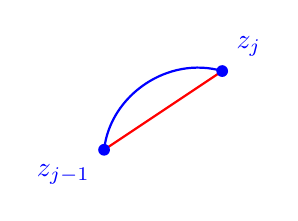
\begin{tikzpicture}[
    dot/.style={fill=blue, circle, inner sep=1.5pt}, % Blue dots
    labelstyle/.style={blue} % Blue labels
]

    % Define Coordinates (adjust spacing/angle as needed)
    \coordinate (zj_minus_1) at (0, 0);
    \coordinate (zj) at (1.5, 1);

    % Draw Straight Red Line
    \draw[red, thick] (zj_minus_1) -- (zj);

    % Draw Curved Blue Arc
    % 'bend left' creates an arc curving upwards between the points
    % Adjust the angle (e.g., 50) to change the curvature
    \draw[blue, thick] (zj_minus_1) to[bend left=50] (zj);

    % Draw Points and Labels (draw last to be on top)
    \node[dot, label={[labelstyle]below left:$z_{j-1}$}] at (zj_minus_1) {};
    \node[dot, label={[labelstyle]above right:$z_j$}] at (zj) {};

\end{tikzpicture}
\end{document}